\chapter{Methodology}\label{ch:3}
This chapter delineates the comprehensive and systematic methodology employed to develop and evaluate a sophisticated classification pipeline capable of determining course equivalency from domain-specific textual data. The methodological framework presented here is the result of an evolutionary research process that progressed through two distinct phases. The investigation commenced with an initial, exploratory phase to assess the feasibility of using Large Language Models (LLMs) as end-to-end classifiers for the task. This direct approach was conceived as an initial benchmark, leveraging a small, manually curated dataset while a larger, more comprehensive dataset was anticipated but not yet available.

In this first phase, the LLM was treated as a holistic reasoning engine, responsible for the entire classification process from raw text input to a final equivalency judgment. The findings from this stage were critical; they demonstrated the potential of modern LLMs but also highlighted significant limitations, including high sensitivity to prompt engineering and the absence of fine-grained similarity metrics for nuanced comparisons. These challenges fundamentally shaped the subsequent research, motivating the development of a more robust and scalable framework.

Consequently, the primary focus of this thesis is a more advanced, decoupled methodology designed specifically to overcome the drawbacks of the direct classification approach. The foundational principle of this final pipeline is to utilize state-of-the-art deep embedding models not as end-to-end classifiers, but as highly sophisticated feature extraction engines. In this paradigm, each course description is converted into a high-dimensional numerical vector that encapsulates its rich semantic content. By pre-processing and storing these embeddings, the framework eliminates the need to repeatedly process raw text through costly APIs, drastically reducing computational overhead and making the system inherently more scalable and suitable for real-world applications.

The narrative of this chapter follows this logical and chronological evolution, detailing the data acquisition, model architectures, training protocols, and evaluation frameworks for each stage of the research. We begin by examining the initial direct LLM classification approach, its implementation, and the key findings that paved the way for the more advanced methods that followed.

\section{Initial Approach: Direct LLM Classification}\label{ch:3.1}
The research commenced with an exploratory phase designed to determine the feasibility of leveraging Large Language Models (LLMs) as end-to-end classifiers for the course equivalency task. This direct approach was a pragmatic first step, conceived as an initial benchmark to establish a baseline for performance using a small, manually curated dataset. At this stage of the research, a larger, more comprehensive dataset from the Program Pathways Mapper (PPM) was anticipated but not yet available, making a focused, smaller-scale investigation the most logical starting point. This methodology treated the LLM as a holistic reasoning engine, tasked with performing the entire classification from raw text input to a final equivalency judgment without intermediate feature engineering. The findings from this initial stage were critical, as they highlighted both the potential and the inherent limitations of direct LLM classification, thereby fundamentally shaping the development of the more complex, decoupled pipeline that followed.

\subsection{Initial Data Corpus and Pre-processing}
The dataset for this initial evaluation was constructed to represent a challenging, real-world scenario using publicly available data. The process began by identifying five required lower-division courses for the Computer Science major at San Francisco State University (SFSU). Using ASSIST, articulation agreements were found for these courses across 63 different California public colleges and universities. The raw course data was then manually collected from the online course catalogs of each respective college. This data was consisted of the full, unmodified text including department codes, course numbers, titles, descriptions, and all associated metadata such as prerequisites, unit counts, and grading options. This approach was deliberately chosen to ensure that the analysis could compare the effectiveness of classification using the complete raw text versus more structured, extracted information.

The initial dataset consisted of 228 equivalent course pairs based on the articulation agreements. To create a more robust dataset for binary classification, this set was expanded by assuming symmetry and transitivity for course equivalency, which generated a total of 5,660 equivalent pairs. An equivalent number of non-equivalent pairs was then generated by randomly pairing courses from different subjects. From this expanded corpus of over 11,000 pairs, a final stratified random sample of 400 pairs (200 equivalent and 200 non-equivalent) was created to serve as the evaluation set for the models.

\subsection{Model Selection and Prompt Engineering}
An initial review of various LLMs was conducted to assess their ability to reliably generate structured data from the raw course descriptions. While many open-source and proprietary models were tested, Google's PaLM2 and its successor, Gemini Pro v1.0, were ultimately selected for this phase of the research. This decision was based on their accessibility via a free-tier API and, most importantly, their consistent ability to produce well-formatted, structured data from the unprocessed text.

A systematic, iterative prompt engineering process, illustrated by Figure~\ref{fig:prompt_engineering_process}, was employed to develop effective prompts for both the extraction of structured data (like course topics) and the final equivalency classification. This process involved starting with simple prompts and gradually refining them based on established design principles from natural language processing research and community guides~\cite{ye2024promptengineeringpromptengineer,ppp,peg}. The final prompts for data extraction were highly structured, consisting of five parts: a preamble summarizing the task, the raw course data, specific formatting instructions, a JSON model schema defining the desired output, and a postamble with additional clarifying instructions. Despite this careful refinement, the structured data extraction process, particularly for deducing course topics, remained a significant challenge and was prone to occasional contextual errors.
\begin{figure}[tb]
    \captionsetup{skip=5pt}
    \centering
    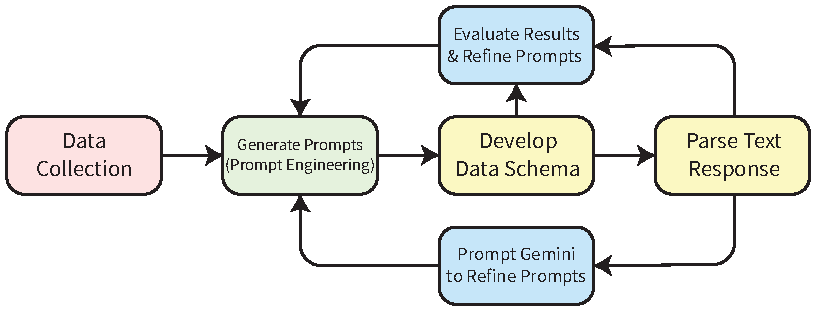
\includegraphics[scale=1,trim={0 0 0 0},clip]{pef.pdf}
    \caption{Prompt Engineering Process}
    \label{fig:prompt_engineering_process}
\end{figure}

\subsection{Classification and Evaluation Findings}
The core of this initial research phase involved pairwise course assessments using Gemini Pro with the previously developed prompts. The evaluation was structured to explore different classification scenarios to gain a comprehensive understanding of the model's capabilities:
\begin{itemize}
    \item \textbf{Input Data}: Evaluations were conducted using both the full, raw course description text and a structured format using only the course discipline and the topics extracted by the LLM.\@
    \item \textbf{Classification Tasks}: Three distinct classification tasks were designed to simulate the complexities of human decision-making: a standard binary classification (``equivalent'' vs. ``non-equivalent''), a three-class model that added an ``unsure'' category for ambiguous cases, and a four-class model that also included an ``insufficient data'' category.
\end{itemize}
The evaluation yielded promising results, with the model achieving a notable 90.5\% accuracy on the binary classification task when using the full raw text. This result confirmed that the unprocessed text was a superior input format, as performance degraded significantly when using only the structured topics, possibly due to the minor but persistent errors introduced during the LLM's extraction process. Furthermore, the experiments that introduced ``unsure'' and ``insufficient data'' categories also proved valuable. While these classifications cannot be measured against a ground truth, they successfully simulated the ambiguity a human advisor might face and demonstrated a method for isolating cases that would require further manual review.

Crucially, this initial investigation revealed several fundamental weaknesses in the direct LLM approach, making it unsuitable for a scalable, reliable production system. The method provided no confidence scores for its decisions, leaving the end-user with a ``black box'' judgment without any measure of certainty. It also lacked a granular similarity metric, preventing the system from ranking different course pairs or identifying courses that are ``close but not equivalent''. The approach was also computationally expensive due to the significant token input required for every single pairwise comparison. Finally, the prompts were found to be highly model-specific, which would lead to significant rework if the underlying model were ever updated or changed. These limitations directly motivated a pivot in methodology towards the decoupled, embedding-based pipeline. This new approach was first developed and prototyped using the initial, manually-curated dataset. The following sections will now detail this final, more robust methodology, beginning with the larger and more comprehensive data corpus upon which it was ultimately trained and validated.

\section{The PPM Corpus and Data Preparation}\label{ch:3.2}
The limitations identified in the initial study necessitated not only a more sophisticated methodology but also a larger, more comprehensive dataset to robustly train and evaluate it. This required data corpus was procured at a later stage of the research in partnership with the Program Pathways Mapper (PPM). The acquisition of this dataset was a critical step that enabled the full-scale implementation and validation of the decoupled pipeline. This section characterizes this final PPM data corpus and details the preparation steps undertaken before its use in the model fine-tuning and evaluation stages described later in this chapter.

\subsection{Dataset Characterization and Partitioning}\label{ch:3.2.1}
The corpus provided by the PPM initially contained 2,217 courses, each labeled with a Course Identification Numbering System (C-ID) code that serves as the ground truth for course equivalency. To prepare this data for a robust, stratified partitioning, a critical filtering step was applied first. All C-ID classes with fewer than four associated courses were removed from the dataset. This step was essential to guarantee that after splitting the data, both the training and subsequent test sets would contain enough examples to form at least one equivalent course pair for every class, a necessary condition for the fine-tuning process. This filtering resulted in a final, clean corpus of 2,157 courses distributed across 157 distinct C-ID classes

To ensure a rigorous and unbiased evaluation of the final models, this final dataset was partitioned into two distinct, non-overlapping subsets: a training set and a test set. A stratified 50/50 split was employed, using the C-ID code as the stratification key. This resulted in a training set of 1078 courses and a test set of 1079 courses. The stratification ensures that each of the 157 classes is represented in both subsets, with each class containing between 2 and 33 equivalent courses per set.  The test set is held in reserve and used only once for the final, conclusive evaluation of the optimized classification pipeline, providing an honest estimate of the model's generalization performance on unseen data.

The training set serves a dual purpose in this methodology, a strategy made possible by the different data formats required by the training and validation procedures. For the fine-tuning process itself, the training set is used to generate (anchor, positive, negative) triplets as required by the Triplet Loss objective. For the validation within the fine-tuning process, this same training set is utilized to generate binary pairs of ``equivalent'' and ``non-equivalent'' course pairs. This validation set is then used with the \verb|BinaryClassificationEvaluator| to monitor model performance during training and select the best model checkpoint. This approach allows for robust validation without data leakage, as the model is evaluated on our primary task (binary pair classification) rather than the one it is directly optimizing for (triplet distance minimization).

\subsection{Input Document Normalization}
In a departure from conventional NLP pipelines, this research deliberately eschewed standard text pre-processing techniques such as lowercasing, stop-word removal, or the stripping of special characters. This decision was made to more accurately simulate a real-world use case where input data, such as course information copied directly from a university website, may be imperfectly formatted or contain extraneous characters. The methodology, therefore, relies on the inherent semantic power and robustness of modern transformer-based embedding models to interpret and handle this ``raw'' text.

Instead of cleaning the text, a normalization step was performed to create a consistent, structured input document for the embedding models. A new field, ``Formatted Course Info,'' was generated for each course by concatenating four key pieces of information: the department name, the department course number, the course title, and the full course description. For example, a course might be transformed into the following single string:
\begin{lstlisting}
    
\end{lstlisting}
This concatenated string serves as the single document representation for each course and is the direct input for the document embedding process. This approach ensures that all relevant textual context is preserved in a standardized format before being converted into a numerical vector.

\subsection{Data Structuring for Fine-Tuning}\label{ss:datastructure}
While the previous subsection defined the content of each input document, this section details how those documents are structured and batched to meet the specific requirements of the chosen fine-tuning objective. The family of triplet loss functions used in this research operates on a conceptual structure of (anchor, positive, negative) triplets~\cite{reimers-2019-sentence-bert,sbertLossOverview}. A key advantage of the batch-based triplet loss functions is that they do not require the manual, pre-generation of these triplets; instead, the loss function intelligently forms the necessary triplets on-the-fly from within each mini-batch of (text, label) pairs.~\cite{sbertLossOverview}.

A crucial constraint imposed by triplet loss functions, particularly those available in the sentence-transformers library, is that the training data must contain a minimum of two examples for each class label~\cite{sbertLosses}. This is not a superficial requirement but a fundamental necessity for the loss computation to be valid. The formation of an (anchor, positive) pair requires selecting two distinct samples from the same class~\cite{sbertLosses}. If a class is represented by only one sample, it can never form a positive pair and can only contribute to (anchor, negative) pairings.

This constraint has a direct and significant implication for the data loading and batching strategy. A simple random sampling approach could easily result in mini-batches that lack the necessary class diversity, containing only one or even zero instances of certain classes. In such a scenario, no valid triplets could be formed for the anchors of those underrepresented classes within that batch, leading to an inefficient and potentially biased training process. To mitigate this, a more sophisticated data loading mechanism was required. Rather than implementing a fully custom solution, this research leveraged a specialized, built-in feature of the sentence-transformers library: the \verb|GroupByLabelBatchSampler|. This sampler, activated by setting the \verb|batch_sampler| argument to \verb|BatchSamplers.GROUP_BY_LABEL| during trainer configuration, is specifically designed for use with triplet loss functions~\cite{sbertSamplers}. It addresses the sampling challenge by ensuring that each mini-batch is constructed by grouping samples with the same label, thereby guaranteeing that every batch contains the necessary class diversity to form valid and informative triplets for all anchors. This demonstrates a key principle of the methodology: the data preparation and loading stage is not an independent preliminary step but is intrinsically linked to and constrained by the fine-tuning objective.

\section{Embedding Model Selection and Fine-Tuning}\label{ch:3.3}
A central hypothesis of this research is that a generic, pre-trained deep embedding model can be adapted to produce highly specialized and semantically rich embeddings for the specific domain of the data corpus. These bespoke embeddings are expected to provide a more discriminative feature representation for downstream classification tasks compared to off-the-shelf embeddings. This section details the architecture, learning objective, and training protocol used to achieve this adaptation through a process of deep metric learning.

\subsection{Model Selection}
The selection of an appropriate embedding model is a critical first step that influences the entire downstream pipeline. Rather than committing to a single model, this research began with a broad preliminary analysis of a variety of open-source embedding models to identify strong candidates for a more in-depth, comparative study. The initial models reviewed, summarized in Table~\ref{tbl:emb_models}, spanned a wide range of parameter sizes and characteristics.
\begin{table}[!tb]
    \captionsetup{skip=5pt}
    \centering
    % \renewcommand{\arraystretch}{1.2}  % Provide more space between table rows, if you prefer
    \caption{Initial Embedding Model Review}
    \label{tbl:emb_models}
    % \resizebox{\columnwidth}{!}{
    \begin{tabular}{lcccc}
        \toprule
        Model Name                 & Rank$^{*}$ & Params$^{\dagger}$ & Dims & Acc             \\
        \midrule
        GIST-small-Embedding-v0    & 41         & 33                 & 384  & 0.9759          \\
        bge-small-en-v1.5          & 47         & 33                 & 384  & 0.9670          \\
        GIST-Embedding-v0          & 33         & 109                & 768  & 0.9768          \\
        bge-base-en-v1.5           & 35         & 109                & 768  & 0.9732          \\
        gte-base-en-v1.5           & 31         & 137                & 768  & 0.9732          \\
        mxbai-embed-large-v1       & 24         & 335                & 1024 & 0.9759          \\
        gte-large-en-v1.5          & 21         & 434                & 1024 & 0.9777          \\
        multilingual-e5-large-inst & 34         & 560                & 514  & 0.9670          \\
        stella\_en\_1.5B\_v5       & 3          & 1543               & 8192 & 0.9857          \\
        SFR-Embedding-2\_R         & 4          & 7111               & 4096 & \textbf{0.9839} \\
        Agte-Qwen2-7B-instruct     & 5          & 7613               & 3584 & 0.9804          \\
        nvidia/NV-Embed-v2         & 1          & 7851               & 4096 & 0.9831          \\
        \bottomrule
        \multicolumn{4}{p{6cm}}{\scriptsize $^{*}$ Huggingface Overall Leaderboard Rank}      \\
        \multicolumn{4}{p{6cm}}{\scriptsize $^{\dagger}$ in Millions}
    \end{tabular}
    % }
\end{table}

To screen these models efficiently, the simple but effective cosine similarity accuracy metric was used: for a given anchor course, a model was considered correct if the cosine similarity to an equivalent course was greater than the similarity to a non-equivalent course. Sufficient to narrow down the field without the computational expense of a full classification pipeline for every single model, this method allowed for the rapid elimination of poorly performing models. This initial screening revealed that while performance varied, many models achieved high accuracy, with a sample mean of \(0.9767\) and a standard deviation of \(0.00605\). Based on these results and a desire to evaluate a representative spectrum of model sizes, three models were selected for the primary analysis:
\begin{itemize}
    \item \verb|BAAI/bge-small-en-v1.5| (BGE): Representing a high-performing small model;
    \item \verb|avsolatorio/GIST-Embedding-v0| (GIST): Representing a medium-sized model; and
    \item \verb|nvidia/NV-Embed-v2| (NVE): Representing a large-scale model.
\end{itemize}

At a later stage of the research, \verb|Salesforce/SFR-Embedding-2_R| (SFR) was also included for additional comparison due to its strong performance on public leaderboards. The foundational architecture for all these models is the transformer, which allows them to generate rich, contextual embeddings. By employing a pooling layer (typically mean-pooling), these models produce a single, fixed-size vector for each input document, making them highly suitable for feature extraction.

\subsection{Metric Learning with Batch Triplet Loss Functions}
To determine if performance could be further improved, BGE was subjected to a fine-tuning process using a metric learning approach. Metric learning aims to learn an embedding space where the geometric distance between samples corresponds to their semantic similarity.  One of the central hypotheses of our research is that a generic, pre-trained model can be adapted to produce highly specialized and semantically rich embeddings specifically for the domain of course descriptions, which could perform better than strong off-the-shelf models.

\subsubsection{Theoretical Foundation of Triplet Loss}
The concept of Triplet Loss was first introduced by Yu, et al. in the context of face recognition and has since been widely applied to supervised similarity learning~\cite{Yu2020}. It operates on the (Anchor, Positive, Negative) triplets described in Section~\ref{ss:datastructure}. The fundamental goal of Triplet Loss is to train the embedding function, \(f(x)\), to map inputs into a vector space where the distance between an anchor sample (\(A\)) and a positive sample (\(P\)) from the same class is smaller than the distance between the anchor and a negative sample (\(N\)) from a different class. To prevent the model from collapsing all embeddings to a single point and to ensure a meaningful separation, the loss function enforces a margin, \(\alpha\). The distance between the anchor-positive pair must be smaller than the distance to the anchor-negative pair by at least this margin.

The mathematical formulation of the Triplet Loss is given by:
\[ L(A,P,N)=\max(d(f(A),f(P))-d(f(A),f(N))+\alpha,0). \]
Here, \(d\) represents a distance metric, which in this study is the Euclidean distance. The \(\max(d(f(A),f(P))-d(f(A),f(N))+\alpha,0)\) component ensures that the loss is only incurred for triplets that violate the margin constraint. If the negative sample is already further from the anchor than the positive sample by at least the margin, the loss for that triplet is zero, and no weight update is performed.

In the context of this research, metric learning, and more specifically Triplet Loss, provides a more powerful and nuanced objective than simple classification.  This directly addresses one of the key limitations of the direct LLM classification approach, which expressly lacked this metric for comparing different course pairs.

\subsubsection{Online Triplet Mining and Batch-based Losses}
A naive implementation of Triplet Loss would form all possible triplets from the training data, an approach known as ``offline'' mining. This is computationally infeasible for large datasets and highly inefficient, as the vast majority of triplets are ``easy'' and provide no useful learning signal. A more effective approach is ``online'' mining, where informative triplets are selected on-the-fly from within each mini-batch of training data. Within this paradigm, triplets can be categorized by their difficulty :
\begin{itemize}
    \item \textbf{Easy Triplets}: These triplets already satisfy the margin constraint, i.e., \(d(A,P)+\alpha<d(A,N)\). They result in zero loss and do not contribute to learning.
    \item \textbf{Semi-Hard Triplets}: In these triplets, the negative sample is more distant than the positive sample but still lies within the margin, i.e., \(d(A,P)<d(A,N)<d(A,P)+\alpha\). These triplets have a positive loss and provide a useful, stable gradient for training.
    \item \textbf{Hard Triplets}: These are the most challenging cases, where the negative sample is closer to the anchor than the positive sample, i.e., \(d(A,N)<d(A,P)\). These triplets produce the largest loss values and provide the strongest learning signal, forcing the model to learn fine-grained distinctions.
\end{itemize}

\subsubsection{Empirical Evaluation of Batch Triplet Loss Functions}
Recognizing that different triplet mining strategies can significantly impact model performance, this research empirically evaluated all four primary batch-based triplet loss implementations available in the sentence-transformers library to identify the optimal strategy for this specific dataset and task. This approach ensures that the chosen loss function is best suited to the data's characteristics, rather than relying on a single, pre-selected method. The evaluated loss functions were:
\begin{itemize}
    \item \textbf{BatchAllTripletLoss}: This function computes the loss for all valid triplets that can be formed within a given batch. While this approach is comprehensive, it can be computationally intensive, and the learning signal can be diluted by the high number of ``easy'' triplets that contribute zero to the loss.
    \item \textbf{BatchSemiHardTripletLoss}: This function focuses the training effort by considering only semi-hard triplets for each anchor. This is a common strategy that provides stable training but can sometimes lead to slower convergence as it ignores the most challenging ``hard'' examples that often provide the strongest learning signal.
    \item \textbf{BatchHardTripletLoss}: This function implements a more aggressive mining strategy. For each anchor sample in a mini-batch, it identifies the hardest positive (the positive sample that is furthest away) and the hardest negative (the negative sample that is closest). The loss is then computed on these most challenging pairs. This can accelerate convergence but is also known to be ``temperamental,'' potentially leading to a noisy and difficult optimization landscape.
    \item \textbf{BatchHardSoftMarginTripletLoss}: This function is a variation of \verb|BatchHardTripletLoss| that also focuses on the hardest positive and negative samples but does not require a manually specified margin parameter. This simplifies hyperparameter tuning while still leveraging an aggressive mining strategy.
\end{itemize}
Because different mining strategies can significantly impact final model performance, all four implementations were empirically tested to identify the optimal strategy for this specific dataset and task. The final model used for feature generation was trained with the loss function that demonstrated the best performance on the validation set during this empirical evaluation.

\subsection{Optimization and Training Protocol}
The successful fine-tuning of a model with a challenging objective like \verb|BatchHardTripletLoss| is critically dependent on the choice of optimizer and learning rate schedule. The components selected for this research, AdamW and Cosine Annealing with Warm Restarts, were not chosen in isolation but as parts of a cohesive, synergistic framework designed to ensure stable and effective learning.

\subsubsection{Optimizer Selection: AdamW}
The optimization of the model's weights was performed using the AdamW optimizer. The foundation of AdamW is the Adam (Adaptive Moment Estimation) optimizer, which has become a de facto standard in deep learning due to its computational efficiency and effectiveness. Adam combines the benefits of two other optimization algorithms: the momentum method, which helps accelerate gradient descent in the relevant direction, and RMSprop, which adapts the learning rate for each parameter based on the magnitude of past gradients. This per-parameter adaptive learning rate makes Adam particularly well-suited for the noisy gradients that can arise from \verb|BatchHardTripletLoss|.

However, the standard implementation of Adam has a subtle flaw in how it handles L2 regularization, also known as weight decay. In standard Adam, the weight decay term is coupled with the gradient update itself. This means that the regularization effect is influenced by the magnitude of the gradient, leading to an inconsistent application of weight decay. For parameters with large gradients, the effective weight decay is reduced, which can hinder proper regularization and lead to poorer generalization~\cite{loshchilov2019decoupledweightdecayregularization}.

AdamW, proposed by Loshchilov and Hutter, corrects this flaw by decoupling the weight decay from the gradient update step. The adaptive moment updates are performed as in standard Adam, but the weight decay is applied as a separate, final step, directly modifying the weights. This decoupled approach ensures that weight decay acts as a true regularizer, penalizing large weights uniformly without interfering with the optimizer's adaptive learning mechanism. For a complex and potentially unstable training process like the one employed here, the enhanced generalization and training stability offered by AdamW make it a superior choice over standard Adam~\cite{loshchilov2019decoupledweightdecayregularization}. It provides the necessary regularization to prevent overfitting on the ``hard'' examples mined by the loss function, while preserving the adaptive learning that helps navigate the complex loss surface.

\subsubsection{Learning Rate Schedule: Cosine Annealing with Warm Restarts}
Static or linear learning rates are often suboptimal for training deep neural networks. A global learning rate schedule, which dynamically adjusts the learning rate during training, can significantly improve convergence and final model performance, even when using an adaptive gradient algorithm such as AdamW~\cite{loshchilov2019decoupledweightdecayregularization}. For this research, the \verb|CosineAnnealingWarmRestarts| schedule was employed. This schedule combines two powerful concepts: cosine annealing and warm restarts. Cosine annealing smoothly decays the learning rate from an initial maximum value, \(\nu_{\textrm{max}}\), to a minimum value, \(\nu_{\textrm{min}}\), following the shape of a cosine curve. The learning rate \(\nu_t\) at a given epoch \(T_{\textrm{cur}}\) within a cycle of length \(T_i\) is calculated as:
\[ \nu_t = \nu_{\textrm{min}} + \frac{1}{2}\left( \nu_{\textrm{max}} -\nu_{\textrm{min}} \right)\left(1 + \cos\left(\frac{T_{\textrm{cur}}}{T_{\textrm{max}}}\pi\right)\right) \]
This smooth, gradual decay is often more effective than abrupt step-wise decays, allowing the model to fine-tune its parameters more carefully as it approaches a minimum in the loss landscape~\cite{pytorchcosanneal}.  The warm restarts technique introduces periodic ``restarts'' into the training process. After a specified number of epochs, \(T_0\), the learning rate is abruptly reset to its initial maximum value, \(\nu_{\textrm{max}}\), and the cosine decay cycle begins anew. The length of subsequent cycles can be progressively increased by a multiplicative factor, \(T_{\textrm{mult}}\).  For example, if \(T_0 = 10\) and \(T_{\textrm{mult}}=2\), the restarts would occur after 10, 30 (10+20), 70 (10+20+40), and so on, epochs.

The combination of these two techniques forms a powerful optimization strategy. The aggressive nature of \verb|BatchHardTripletLoss| creates a complex loss surface with many sharp, suboptimal local minima. A standard decay schedule might cause the optimizer to converge into one of these minima and become stuck. The ``warm restarts'' provide a crucial escape mechanism. When the model's performance on the validation set begins to plateau, suggesting convergence into a local minimum, the sudden increase in the learning rate effectively ``kicks'' the optimizer out of that basin, allowing it to explore other regions of the loss landscape. The subsequent smooth cosine decay then enables the optimizer to carefully descend into any new, potentially broader and deeper, minimum it discovers.

This entire fine-tuning framework (\verb|BatchHardTripletLoss|, \verb|AdamW|, and \verb|CosineAnnealingWarmRestarts|) represents a carefully orchestrated system. The loss function provides a powerful, albeit challenging, learning signal. The optimizer provides a stable, well-regularized mechanism for applying weight updates based on that signal. The learning rate schedule provides a global exploration strategy to guide the optimizer across the complex landscape, preventing premature convergence and increasing the likelihood of finding a high-quality solution. This synergistic design is critical for successfully training a highly discriminative embedding model under these demanding conditions.

\section{Generating Course Embeddings}
Upon completion of the model selection and fine-tuning processes, the next stage of the methodology involves using the selected models to transform the entire text corpus into structured numerical formats suitable for a comparative analysis of downstream machine learning classifiers.

This process was executed by loading each selected embedding model and operating it in inference mode. The ``Formatted Course Info'' text for each course in the training and test sets was individually fed into each model to generate a fixed length embedding vector. This procedure was performed for the models summarized in Table~\ref{tbl:emb}.
\begin{table}[!bt]
    \captionsetup{skip=5pt}
    \caption{Embedding Models \& PCA Explained Variance}
    \centering
    \resizebox{\columnwidth}{!}{
        \begin{tabular}{lcp{9em}p{5em}p{2.2em}p{2.2em}p{2.2em}}
            \toprule
                                        &           &                            &                       & \multicolumn{3}{c}{Explained Variance}               \\
                                        &           & \centering\# of Parameters & \centering Embedding  & \multicolumn{3}{c}{(\# of PCs)}                      \\
            \cmidrule{5-7} Model Name     & Type Used\(^{*}\) & \centering (in Millions)   & \centering Dimensions & 70\%                                   & 80\% & 90\% \\
            \midrule
            BAAI/bge-small-en-v1.5        & OTS \& FT & \centering 33              & \centering 384        & 28                                     & 45   & 76   \\
            avsolatorio/GIST-Embedding-v0 & OTS \& FT & \centering 109             & \centering 768        & 23                                     & 40   & 73   \\
            nvidia/NV-Embed-v2            & OTS       & \centering 7851            & \centering 4096       & 20                                     & 37   & 73   \\
            Salesforce/SFR-Embedding-2\_R  & OTS       & \centering 7111            & \centering 4096       & 20                                     & 37   & 73   \\
            \bottomrule
            \multicolumn{4}{p{6cm}}{\scriptsize \(^{*}\) OTS: Off-The-Shelf; FT: Fine-Tuned}
        \end{tabular}
    }
    \label{tbl:emb}
\end{table}

The outcome of this procedure is the creation of multiple distinct sets of numerical matrices (one for the training set and one for the test set per embedding model). In each matrix, every row corresponds to a specific text sample from the original corpus, and the columns represent the dimensions of that model's embedding space. These matrices, along with their corresponding class labels, constitute the final feature sets that serve as the direct input for the suite of classification models evaluated in the next section. This step marks the critical transition from the unstructured domain of natural language processing to the structured domain of tabular data analysis, upon which the final classification experiments are built.

\section{Feature Vector Construction}
The high-dimensional embedding vectors generated in the previous step, while semantically rich, are not the final features used for classification. To prepare the data for the downstream classifiers, a two-stage feature engineering pipeline was executed. This pipeline first applies various dimensionality reduction techniques to the embeddings and then constructs pairwise difference vectors from these reduced (and original) embeddings to explicitly represent the relationship between two courses for the equivalency classification task.

\subsection{Dimensionality Reduction}
The high-dimensional vectors produced by modern embedding models, while semantically rich, can present challenges for downstream machine learning algorithms, a phenomenon often referred to as the ``curse of dimensionality.'' In this high-dimensional space, the data becomes extremely sparse, which can make it more difficult for some algorithms to discern meaningful patterns and can increase the risk of the model overfitting to noise in the training data. To address these potential issues, a systematic process of dimensionality reduction was applied to the embeddings generated by each model.

This investigation was motivated by several potential benefits. First, by reducing the number of features, we can sometimes improve a model's ability to generalize to unseen data. This is achieved by removing redundant or noisy dimensions, forcing the classifier to learn from the most salient and robust features in the data. Second, a reduction in dimensionality leads to a direct reduction in computational complexity. Fewer dimensions mean that the downstream classifiers require less memory and can be trained and evaluated more quickly, which is a significant practical advantage for both experimentation and potential production deployment. Together, these benefits serve to mitigate the curse of dimensionality, making the classification task more tractable.

To ensure the integrity of the evaluation and prevent any form of data leakage, the reduction models were governed by a strict protocol. Using a dedicated EmbeddingReducer class, each reduction technique was fit exclusively on the training data. The same fitted model was then used to transform both the training and the held-out test sets. This methodology guarantees that no information from the test set influences the parameters of the reduction models, ensuring that the final evaluation remains unbiased.

A comprehensive exploration was conducted to determine the optimal dimensionality for the task. This included using Principal Component Analysis (PCA) to reduce the vectors to the number of components required to explain 70\%, 80\%, and 90\% of the original variance. Additionally, to test performance in very low-dimensional spaces, the embeddings were reduced to a static 4 and 7 dimensions using multiple techniques, including PCA, t-SNE, and PaCMAP.  The outcome of this stage was a suite of new training and test matrices for each base embedding model, each corresponding to a unique combination of a reduction technique and a target dimensionality, ready for the next step of feature vector construction.

\subsection{Global and Local Distance Vector}
The ultimate goal of this research is to classify pairs of courses as either “equivalent” or “not equivalent.” This requires input features that represent the relationship between two courses, not just the characteristics of a single one. Our preliminary analysis showed that relying on a single, holistic metric like cosine similarity was insufficient for establishing a clear and reliable decision boundary. To overcome this, we designed a composite feature vector that provides a richer, more discriminative representation of a course pair's relationship.

The feature vector, denoted as \(\Delta_c\), is constructed by concatenating the element-wise difference of the two course embedding vectors (\(\mathbf{A}\) and \(\mathbf{B}\)) with their cosine similarity. The formal definition is as follows:
\[ \Delta_c = \left(a_1 - b_1, \dots, a_k - b_k, \frac{\mathbf{A}\cdot\mathbf{B}}{\parallel \mathbf{A} \parallel \parallel \mathbf{B} \parallel } \right) \]
where \(\mathbf{A} = (a_1, \dots, a_k) \) and \(\mathbf{B} = (b_1, \dots, b_k) \) are the \(k\)-dimensional embedding vectors for the two courses.  This design is powerful because it provides the subsequent classifier with two distinct types of information simultaneously. The element-wise difference captures granular, dimension-specific (local) disparities between the two semantic representations, while the cosine similarity provides a single, normalized measure of their overall (global) alignment in the vector space. This composite vector creates a much more informative and discriminative feature set than a single similarity score alone.

To generate the data for our models, a \verb|CoursePairGenerator| class was implemented. This utility systematically created the training and test datasets by first assembling positive pairs (courses with the same C-ID label) and negative pairs (courses with different C-ID labels). For each of these pairs, it then computed the composite feature vector \(\Delta_c\), resulting in a highly informative and discriminative feature set ready for classification.

This procedure was applied to every set of embeddings (e.g., BGE-original, BGE-PCA4-reduced, GIST-original, etc.), resulting in a comprehensive suite of training and testing datasets. Each dataset corresponds to a unique combination of an embedding model and a dimensionality reduction technique, ready for evaluation by the downstream classifiers detailed in the next section.

\section{Classification Models}
To determine the most effective method for classifying the generated pairwise feature vectors, a broad suite of machine learning algorithms was evaluated. This process began with a comprehensive initial evaluation of eight different models to understand which algorithmic families were best suited to the data. Based on those preliminary results, a smaller, more focused set of high-performing models was selected for the final, in-depth analysis.

\subsection{Initial Evaluation}
The initial evaluation included a diverse set of classifiers, each chosen to test a different hypothesis about the structure of the feature space:
\begin{itemize}
    \item \textbf{Linear Models (Logistic Regression, Ridge, Lasso)}: These models were used to establish a baseline and determine the degree of linear separability of the data. Their simplicity and interpretability make them excellent for understanding the foundational difficulty of the classification task. 
    \item \textbf{Instance-Based Model (k-Nearest Neighbors)}: KNN was included to probe the local structure of the feature space. Its performance indicates whether courses with the same equivalency status form dense, localized clusters.  
    \item \textbf{Kernel-Based Model (Support Vector Machine)}: An SVM with a non-linear kernel was used to test for complex, non-linear decision boundaries that linear models cannot capture.  
    \item \textbf{Ensemble Model (Random Forest)}: Random Forest was chosen for its robustness to overfitting and its ability to capture complex feature interactions by combining the predictions of many decision trees.  
    \item \textbf{Probabilistic Models (LDA and QDA)}: Linear and Quadratic Discriminant Analysis were used to test assumptions about the geometric distribution of the data, specifically whether the classes share a common covariance (LDA) or have unique ones (QDA).   
\end{itemize}

\subsection{Final Classifier Selection}
Based on the preliminary results from the comprehensive evaluation, four models were selected for the final analysis due to their consistently strong performance: K-Nearest Neighbors (KNN), Support Vector Machine (SVM), Random Forest (RF), and XGBoost. XGBoost, a powerful gradient boosting implementation, was added at this stage to include a state-of-the-art boosting algorithm known for its high performance on structured data. These models represent the most promising approaches for this classification task, covering instance-based, maximal-margin, and advanced ensemble methods.

\section{Multi-Stage Evaluation}
A rigorous, multi-stage evaluation framework was designed to systematically narrow down the optimal combination of embedding models, dimensionality reduction techniques, and classifiers.

\subsection{Stage 1: Preliminary Embedding Model Selection}
The process began with a broad analysis of twelve open-source embedding models to identify strong candidates for more intensive study. This initial screening was performed on a small, manually curated dataset. The evaluation metric was a simple accuracy score based on cosine similarity: for a given course, a model was scored as correct if an equivalent course had a higher cosine similarity than a non-equivalent course. This efficient, low-cost evaluation allowed for the rapid elimination of poorly performing models, resulting in the selection of three top candidates representing a range of sizes: BAAI/bge-small-en-v1.5 (BGE), avsolatorio/GIST-Embedding-v0 (GIST), and nvidia/NV-Embed-v2 (NVE).

\subsection{Stage 2: Comprehensive Classifier and Reducer Evaluation}
Using the three selected embedding models and the initial small dataset, a comprehensive GridSearchCV was conducted. This stage systematically tested each embedding model in combination with multiple dimensionality reduction techniques (PCA, t-SNE, and PaCMAP at 4 and 7 dimensions, as well as with 70\%, 80\%, and 90\% explained variance for PCA) and the full suite of eight initial classifiers (Logistic Regression, Ridge, Lasso, KNN, SVM, Random Forest, LDA, and QDA). The goal of this exhaustive search was to identify the most effective downstream classifiers and to understand the impact of dimensionality reduction on performance.

\subsection{Stage 3: Evaluation During Fine-Tuning}
With the larger, more robust PPM dataset, the two most promising non-proprietary models (BAAI/bge-small-en-v1.5 and avsolatorio/GIST-Embedding-v0) were fine-tuned to specialize them for the course equivalency task. To monitor the quality of the learned embeddings during this process, the \verb|BinaryClassificationEvaluator| from the sentence-transformers library was employed. At the end of each training epoch, the evaluator was run on binary-labeled course pairs generated from the training set. The primary metric monitored was Average Precision based on cosine similarity, and the model checkpoint that achieved the highest score on these validation pairs was saved as the best model for that fine-tuning run.

\subsection{Stage 4: Final Downstream Classifier Evaluation}
The final and definitive evaluation was conducted on the held-out test portion of the PPM dataset. This stage used the feature vectors generated from the best-performing embedding models (both the original off-the-shelf versions and the newly fine-tuned versions). These feature sets were then used to train and evaluate the final selection of high-performing classifiers: KNN, Random Forest, SVM, and XGBoost. This ensures an unbiased assessment of the complete pipeline's ability to generalize to new, unseen data. To provide a comprehensive view of model performance, the standard suite of classification metrics was calculated from the confusion matrix: accuracy, precision, recall, and \(F_1\)-Score.

Beyond classification accuracy, the computational efficiency of each model pipeline was assessed by measuring both training and inference times from the hyperparameter cross-validation grid search. While training time provides insight into the resources required to develop a model, inference time is the more critical metric for this research's use case. Inference time directly affects the system's responsiveness and scalability in a production environment, making it a key factor in determining the practical viability of a given solution.

The performance of each of the final classifiers on each of the final feature sets was measured using these metrics. The results of this final evaluation, which form the core findings of this thesis, will be presented and analyzed in the subsequent chapter.